\subsection{关于正测度的像的积分}

设 \(\pi\) 是一个由 T 到 X 中的 \(\mu\) -逆紧映射，并设 \(\nu = \pi(\mu)\) 。应用 §4 的结果，可得到下列命题：

命题 2. --- 对定义在 X 上的每个数值函数 \(f \geqslant 0\) ，

\[
\int^ {\bullet} f (x) d \nu (x) = \int^ {\bullet} f (\pi (t)) d \mu (t).\tag{2}
\]

这由 §4, No.~2 的定理 1 得出。

推论 1. --- 对 X 的每个子集 A ，

\[
\nu^ {\bullet} (\mathrm{A}) = \mu^ {\bullet} \left(\overline {{\pi}} ^ {- 1} (\mathrm{A})\right).
\]

推论 2. --- 为使 X 的一个子集 A 对 \(\nu\) 是局部可忽略的，必须且只须 \(\overline{\pi}^{-1}(\mathrm{A})\) 对 \(\mu\) 是局部可忽略的。

推论 3. --- 若测度 \(\mu\) 集中于一个集 M 上，则 \(\pi(\mu)\) 集中于 \(\pi(M)\) 上。

因为，若 \(\mathrm{N} = \mathrm{X} - \pi(\mathrm{M})\) ，则 \(\overline{\pi}^1(\mathrm{N})\) 与 \(\mathrm{M}\) 不相交，从而是局部 \(\mu\) -可忽略的，于是（推论 2）\(\mathrm{N}\) 是局部 \(\nu\) -可忽略的。

推论 4. --- 设 S 是 \(\mu\) 的支集。若 \(\pi\) 是连续的，则 \(\pi(\mu)\) 的支集是 \(\overline{\pi(S)}\) 。

因为，由推论 3 知 \(\pi(\mu)\) 集中于 \(\pi(S)\) 上，因此若 \(S'\) 是 \(\pi(\mu)\) 的支集，则 \(S' \subset \overline{\pi(S)}\) 。另一方面，\(\overline{\pi}(X - S')\) 是一个局部 \(\mu\) -可忽略的开集（推论 2），从而是 \(\mu\) -可忽略的（Ch. IV, §5, No.~2, 命题 5 的推论 2）。于是 \(\overline{\pi}(X - S') \subset T - S\) ，因而 \(\pi(S) \subset S'\) ，这就证明了推论。

命题 3. --- 为使一个由 X 到拓扑空间 G 中的映射 f 是 ν-可测的，必须且只须 \(f \circ \pi\) 是 μ-可测的。

这是 §4, No.~3 的命题 3 的直接推论。

推论. --- 为使 X 的一个子集 A 是 \(\nu\) -可测的，必须且只须 \(\overline{\pi}^{1}(A)\) 是 \(\mu\) -可测的。

\pandocbounded{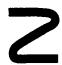
\includegraphics[keepaspectratio]{images/part002_e5542695.jpg}}

然而，\(\pi\) 作用于 T 的一个 \(\mu\) -可测子集 M 所得的像不一定是 \(\nu\) -可测的，即使 \(\pi\) 是连续的且 M 是 \(\mu\) -可忽略的（习题 7 及 §8, 习题 1）。

定理 1. --- 设 f 是定义在 X 上、取值于 \(\overline{R}\) 或一个 Banach 空间 F 中的函数。为使 f 是本质 \(\nu\) -可积的，必须且只须 \(f \circ \pi\) 是本质 \(\mu\) -可积的，此时

\[
\int \mathbf {f} (x) d \nu (x) = \int \mathbf {f} (\pi (t)) d \mu (t).\tag{3}
\]

再设 \(\pi\) 是连续且逆紧的。此时，为使 \(\mathbf{f}\) 是 \(\nu\) -可积的，必须且只须 \(\mathbf{f} \circ \pi\) 是 \(\mu\) -可积的。

只须应用 §4, No.~4 的定理 2。

推论. --- 为使 X 的一个子集 A 是本质 \(\nu\) -可积的，必须且只须 \(\overline{\pi}^{1}(A)\) 是本质 \(\mu\) -可积的，此时 \(\nu(A)=\mu\left(\overline{\pi}^{1}(A)\right)\) 。

特别地，对每个紧集 \(K \subset X\) ，\(\nu(K) = \mu\left(\overline{\pi}(K)\right)\) 。由此以及命题 2 的推论 3 推出：若 \(\mu\) 是原子的（\(\S5\) , No.~10），则 \(\pi(\mu) = \nu\) 也是原子的。因为，设 M 是由 \(t \in T\) （使 \(\mu(\{t\}) \neq 0\) 者）组成的集；由于 \(\mu\) 由 M 承载，\(\nu\) 由 \(\pi(M)\) 承载；此外，对每个 \(x \in \pi(M)\) 有 \(\nu(\{x\}) = \mu\left(\overline{\pi}(x)\right) > 0\) ，因为 \(\overline{\pi}(x)\) 至少含有 M 的一个点。因此 \(\nu\) 是原子的（\(\S5\) , No.~10, 命题 15）。

